\documentclass[conference]{IEEEtran}
\IEEEoverridecommandlockouts
% The preceding line is only needed to identify funding in the first footnote. If that is unneeded, please comment it out.
\usepackage{cite}
\usepackage{amsmath,amssymb,amsfonts}
\usepackage{algorithmic}
\usepackage{graphicx}
\usepackage{textcomp}
\usepackage{xcolor}

\usepackage{hyperref}
\hypersetup{
	colorlinks=true,
	linkcolor=blue,
	filecolor=magenta,      
	urlcolor=cyan,
}
\def\BibTeX{{\rm B\kern-.05em{\sc i\kern-.025em b}\kern-.08em
    T\kern-.1667em\lower.7ex\hbox{E}\kern-.125emX}}
\begin{document}

\title{Blockchain Based Data Storage\\
%{\footnotesize \textsuperscript{*}Note: Sub-titles are not captured in Xplore and
%should not be used}
%\thanks{Identify applicable funding agency here. If none, delete this.}
}

\author{\IEEEauthorblockN{1\textsuperscript{st} Abhiram S}
\IEEEauthorblockA{\textit{Computer Science and Engineering} \\
\textit{Amrita Vishwa Vidyapeetham}\\
Kollam, Kerala, India \\
amenpecse20001@am.students.amrita.edu}
\and
\IEEEauthorblockN{2\textsuperscript{nd} Aiswarya Venugopal}
\IEEEauthorblockA{\textit{Computer Science and Engineering} \\
		\textit{Amrita Vishwa Vidyapeetham}\\
		Kollam, Kerala, India \\
		amenpecse20002@am.students.amrita.edu}
%\and
%\IEEEauthorblockN{3\textsuperscript{rd} Given Name Surname}
%\IEEEauthorblockA{\textit{dept. name of organization (of Aff.)} \\
%\textit{name of organization (of Aff.)}\\
%City, Country \\
%email address or ORCID}
%\and
%\IEEEauthorblockN{4\textsuperscript{th} Given Name Surname}
%\IEEEauthorblockA{\textit{dept. name of organization (of Aff.)} \\
%\textit{name of organization (of Aff.)}\\
%City, Country \\
%email address or ORCID}
%\and
%\IEEEauthorblockN{5\textsuperscript{th} Given Name Surname}
%\IEEEauthorblockA{\textit{dept. name of organization (of Aff.)} \\
%\textit{name of organization (of Aff.)}\\
%City, Country \\
%email address or ORCID}
%\and
%\IEEEauthorblockN{6\textsuperscript{th} Given Name Surname}
%\IEEEauthorblockA{\textit{dept. name of organization (of Aff.)} \\
%\textit{name of organization (of Aff.)}\\
%City, Country \\
%email address or ORCID}
}

\maketitle

\begin{abstract}
With the increasing need to prevent identity theft there is a need for a technology which can easily verify the given data (certificate) as authentic as well as to allow anyone to create an authenticity proof to send or receive data (certificate) from an entity or a person. Blockchain technology can be used in this scenario to prevent the forging of information as well as will give anyone an effortless way to issue or even receive legal documents whose ownership and authenticity can be easily proven to anyone. This needs a way for moving blockchain from the initial application that is cryptocurrency to an idea of securing integrity and authenticity of data.	
\end{abstract}

\begin{IEEEkeywords}
component, formatting, style, styling, insert
\end{IEEEkeywords}

\section{Introduction}
The blockchain is a peer-to-peer distributed ledger in which records called blocks are linked and secure using a crypto- graphic hash. By design, blockchains are decentralized, secure, immutable, and extremely fault tolerance making them suitable for record management activities i.e., financial trans- actions, identity management, provenance, and authentication. In permissionless or public blockchain the actors in the system are not known. Anyone can join or leave the blockchain network at any time, which may raise security risks in the network. However, in permissioned or private blockchain only known and identifiable set of participants are explicitly admitted to the blockchain network. This reduces the presence of malicious actors within the network. As a result, only authenticated and authorized actors can participate in the network which increases the security of the system as required by the enterprise applications. 

Blockchains are write-only data structures with no administrative permissions for editing or deleting of the data. The data structures are known as blocks and are distributed in a P2P network. Each block contains the cryptographic hash function of the previous block and is used to develop a link between them. The linked blocks form a complete chain, hence the term blockchain. The hash function maintains the security, integrity, and immutability of the blockchain. The process of creating new blocks is known as mining. The new blocks are always appended at the end of the blockchain. The main components of the blockchain include Transactions, Blocks, Cryptography, Smart Contracts, Consensus Algorithms, and P2P network. Each component is explained as follows. 
\begin{itemize}
	\item \textbf{Transactions \& Blocks:} The record of an event, cryptographically secured with a digital signature, that is verified, ordered, and bundled together into blocks, form the transactions in the blockchain. Thus, each block is composed of transaction data along with the timestamp, cryptographic hash of the previous block (parent block) and nonce. A nonce is a random number or bit string which is used to verify the hash. The hash values are unique and help to maintain the integrity of the entire blockchain from the first block (genesis block) to the last in the network. 
	
	\item \textbf{Cryptography:} It plays a key role in blockchain by providing the security, immutability and rightful ownership of the transactions being stored on the block. It provides the security and immutability by linking the blocks in a chronological order using the hash function. Note that, the hash only provides the encrypted form of the original transaction from which it is not possible to drive the original transaction data. The examples of hash functions include the family of Secure Hash Algorithms (i.e., SHA1, SHA128, SHA256, SHA512, etc.). The rightful ownership is provided to the transactions using digital signatures. Further, it helps the receiver to verify the authenticity and integrity of the transactions on the network. For example, Bitcoin uses Elliptic Curve Digital Signature Algorithm (ECDSA) based on asymmetric cryptography.
	
	\item \textbf{Smart Contracts: }Nick Szabo coined the term of Smart Contracts for the first time. They are the computer programs that run automatically when certain criteria are met within the system. They are used to transfer value of any kind between the peers in a blockchain without the service of the trusted third party. Today, the Ethereum smart contracts are designed to run on all nodes of the Ethereum network. Similarly, Hyperledger Fabric5 smart contracts are called Chain code. They enable the user to create transactions in the shared ledger of the network. 
	
	\item \textbf{Consensus Algorithms: }They are used in blockchains to achieve the agreement on a single state of the data in       a distributed network. They ensure that the same copy    of the data is available to all peers in the network. Further, they help to prevent the malicious nodes from changing the state of the data in a distributed environment. The consensus algorithms are either lottery-based (Proof of Work, Proof of Elapsed Time) or voting based (Simplified Byzantine Fault Tolerance) depending on the unique requirement of the system and level of fault tolerance. Other available consensus algorithms are Proof of Stake, Proof of Deposit, Proof of Burn etc. 
\end{itemize}
The need for a decentralized authenticity verification and enforcement system has a been around for a long time now. With the creation of blockchain based technology for currency, which is just an application of blockchain, it enabled many more possibilities. Because of the immutability of the chain in a blockchain, it can be easily used for verifying data origin. This means that if government adopts this technology there may be a situation where forging a document may become impossible because the documents integrity is confirmed by blockchain itself which is immutable. This means that, it can well be next age of government where the decision that if a document is valid or not is no longer about holograms and signatures, anyone with the document could check if that document is issued by the correct authority who he/she is claiming to be.  

\section{Related Works}

Nowadays, there are several types of distributed storage systems, such as cloud storage systems, and peer-to-peer (p2p) storage systems. In all these storage systems, data can be stored, archived, and back up over distributed nodes, such as AmazonS3. Users can make use of their stored files any time anywhere; this is an outstanding advantage as to distributed storage systems. There is many research focused on the design and construction of distributed file systems. LIBRY is one of the most popular and successful peer-to-peer distributed file systems and has more than 100 million online users presently. It is a large-scale deployed in which millions of users log-in and log-out every day. Storage resources, as well as system clients in a distributed file system, are scattered in the network. In these systems, users act as both creators and consumers of data, therefore, to provide massive of incentives by a secure and efficient approach. 

Primarily, LBRY is a new protocol that allows anyone to build apps that interact with digital content on the LBRY network. Apps built using the protocol allow creators to upload their work to the LBRY network of hosts (like BitTorrent), to set a price per stream or download (like iTunes) or give it away for free (like YouTube without ads). The work you publish could be videos, audio files, documents, or any other type of file. Traditional video (or other content) sites such as YouTube, Instagram, and Spotify store your uploads on their servers and allow viewers to download them. They also allow creators to make some money through advertising or other mechanisms. However, there are some well-known drawbacks, especially for people whose material is perceived as not being advertiser friendly. LBRY aims to be an alternative to these sites, allowing publishers and their fans to interact directly without the risk of demonetization or other meddling. 

This paper will be suggesting the key areas to which blockchain technology can be made practical in the Decentralized data storage. LBRY like mechanism is used for a decentralized authenticity verification and enforcement system. Like LBRY, Blockchain enables people to create databases that no single entity controls. With Bitcoin, when you send money to someone, your computer broadcasts "hey, the person with this particular secret (a private key) is sending money to that person over there" to the network, and the mining algorithm ensures everyone agrees that indeed, you sent that money, so your balance goes down, and the recipient's goes up. In LBRY, the same mechanism is used to store an index of what content is available and how to download it, as well as financial transactions (such as tips, and purchases of paid content) using the Bitcoin-like currency LBC (LBRY Credits). When a creator publishes something on LBRY, an entry is made on the LBRY blockchain. For the same reasons that nobody can prevent a Bitcoin transaction from taking place, nobody can prevent a transaction (like a publication or a tip) from appearing on the LBRY blockchain. Other sites exist that share their content from a peer-to-peer data network. However, the index of available content is still centralized and can be easily censored. Blockchain technology can be used in this scenario to prevent the forging of information as well as will give anyone an effortless way to issue or even receive legal documents whose ownership and authenticity can be easily proven to anyone. 

Due to issues in integrity, trust, control, and credibility, we focus in this paper on overcoming the issue of integrity and credibility for distributed file storage. There are various systems and platforms for distributed file storage, and they aim to collect all kinds of data. Notably, this incurs a severe privacy problem, since most users have no knowledge of these actions, much less about control of such actions. To solve this problem, we suppose in this work that all provided services should obey the smart contracts, especially some assigned protocols. Our research focuses on the data credibility for distributed file storage; we should guarantee that authorized users must control all personal data. Meanwhile, the systems and platforms regard the services as guests who have corresponding permissions. All data should be verified and detected to guarantee the integrity of stored data. All data-trace is transparent for each authorized user, and any illegal modification is impractical on the platform. Any users should be granted access permission as they log in the system or platform. These permissions should define which resources the users can utilize. Within the permissions, users can change the access range of their stored data. Meanwhile, all participating users must store data access control strategies or policies on the blockchain. Thus, illegal access is hardly impossible. 

\section{Methodology}
Architecture which is followed here is remarkably similar to normal blockchain based cryptocurrencies like bitcoin. As usual there is a Genysis block. This block is the first block that bootstraps the blockchain. Genysis block may or may not contain valid data. This is to allow starting of a blockchain without any transaction. Transactions in this blockchain are files instead of coins. As there are no coins there is no need to keep a double ledger system. This simplifies the blockchain implementation to a point where it is obvious how it is implemented. Transactions need a signature; this is done by the sender using his/her private key. As anonymity is not the goal of this blockchain there is no anonymity. Everyone will be tied to their real identity by their public key. This means that if one person manages to get a random public key, they can verify who this public key belongs to.  

To create a transaction, public key and private key of the sender, public key of the receiver, data to be send and its metadata is needed. Once all these information is given, a transaction can be made. Every transaction will have. 
\begin{enumerate}
	\item Sender Public Key 
	
	\item Receiver Public Key 
	
	\item Timestamp 
	
	\item Meta Data 
	
	\item Data 
	
	\item Signature 
\end{enumerate}
Sender Public Key is the public key of the keypair owned by sender. Receiver Public Key is the public key of the keypair owned by the receiver. Timestamp is the time at which the transaction was made. Metadata contains information about the data which may be useful, metadata contains the “File Name” and the “File Length.” Data is the actual file in raw bytes, data can be at maximum 2MB in size. Signature is the signature of the transaction which is generated by signing a digest of the transaction with private key of the sender.

After 16mb or less amount of data is added into the transaction list, a block is made. For this miner mines the block. For mining, the procedure is same as mining in bitcoin as bitcoin as well as this implementation are both proof of work, that means that every miner tries to find the correct nonce for which the hash value of the block is less than that of the difficulty value. Once a block is mined, as usual, it is broadcasted to every other node so that.  

\begin{figure}[h!]
	\centering
	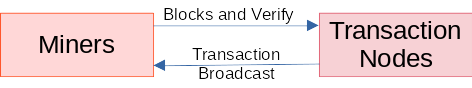
\includegraphics[width=0.7\linewidth]{BlockBroadCast}
	\caption{Miner Node and Transnational Node communication}
	\label{fig:blockbroadcast}
\end{figure}

\begin{enumerate}
	\item Nodes can add the block into its own chain. 
	
	\item Miners can know that one other miner has already won the puzzle. 
\end{enumerate}
Difficulty of the network is set such that a maximum of 1 block is mined per 10 second window. This makes block rate of the blockchain to be 6 blocks per minute. 	
Structure of the block is. 
\begin{enumerate}
	\item Header 
	
	\item Transaction List 
	
	\item Transaction Counter
\end{enumerate}
Structure of the block header is. 
\begin{enumerate}
	\item ID, identification serial number of the block. 
	
	\item Version of the miner with which the block was created. 
	
	\item Previous Block Hash, this contains the hash of the block which comes before the current block. 
	
	\item Merkle Root Hash, this contains the hash of all the transactions abstracted to mrkle root. 
	
	\item Timestamp contains the information of the time when the block was initially created. 
	
	\item Difficulty contains the difficulty of the network when the block was mined. 
	
	\item Nonce is added to the block so that proof of work can function. 
\end{enumerate}




Synchronization mechanism is same as that of the bitcoin. Nodes communicate with each other via gossip protocol as well as nodes can ask each other nodes to get the blocks or understand the consistency of blockchain. All this communication is done with the help of HTTP GET and POST requests which is basics of REST full API. Nodes discover each other also via gossips about the nodes the other nodes know. This means that without much conversation between nodes a node is eventually able to be consistent with other nodes which exist in the network. 

Validation of the blocks is done by reading and checking the consistency of the chain by verifying hashes and signatures of the blocks as well as the transaction, once block is verified and stored, it is never verified again. All nodes do have a copy of the whole block chain, this means that there are no light nodes in the network. As this network is running on proof of work consensus algorithm, if there exist multiple chains the longest chain wins due to maximum work is put into that chain which is harder as the cryptographic puzzles are designed in such a way that it's hard to mine blocks really fast than others. 
\section{Result}
Partial implementation of the system, which is the POC of the system do exist. With the implementation of this about idea it is verified that it will work and therefore is a viable alternative to hologram and other authenticity ensuring mechanism.  
\begin{figure}[h!]
	\centering
	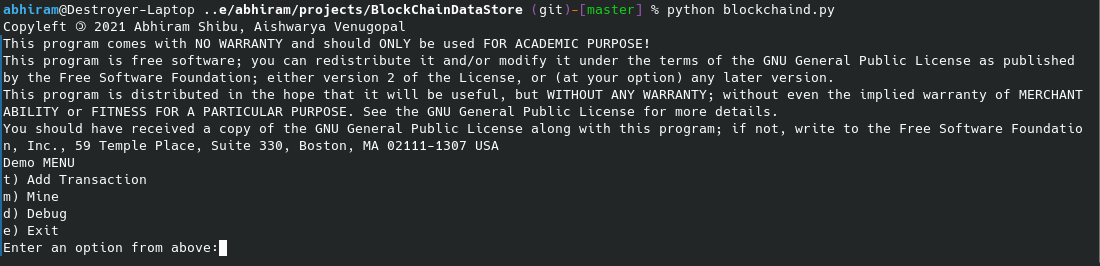
\includegraphics[width=0.7\linewidth]{Menu}
	\caption{Command line menu of the implementation.}
	\label{fig:menu}
\end{figure}
\begin{figure}[h!]
	\centering
	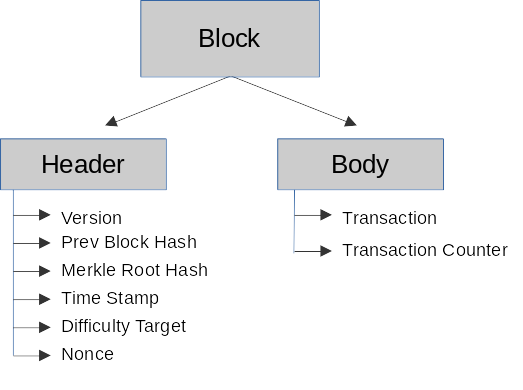
\includegraphics[width=0.7\linewidth]{BlockStructure}
	\caption{Structure of the block}
	\label{fig:blockstructure}
\end{figure}
\begin{figure}[h!]
	\centering
	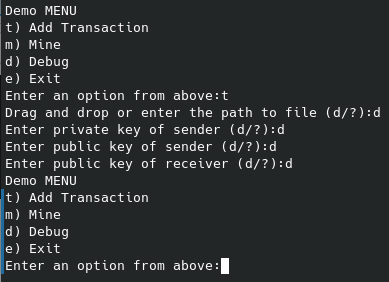
\includegraphics[width=0.7\linewidth]{AddingTransaction}
	\caption{Adding a transaction with defaults}
	\label{fig:addingtransaction}
\end{figure}
\begin{figure}[h!]
	\centering
	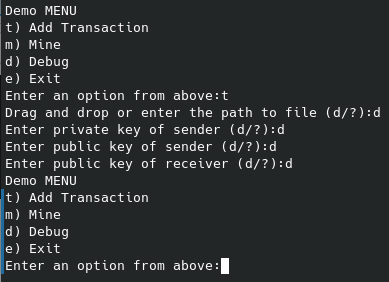
\includegraphics[width=0.7\linewidth]{Mining}
	\caption{Mining Block with command line tool.}
	\label{fig:mining}
\end{figure}
\begin{figure}[h!]
	\centering
	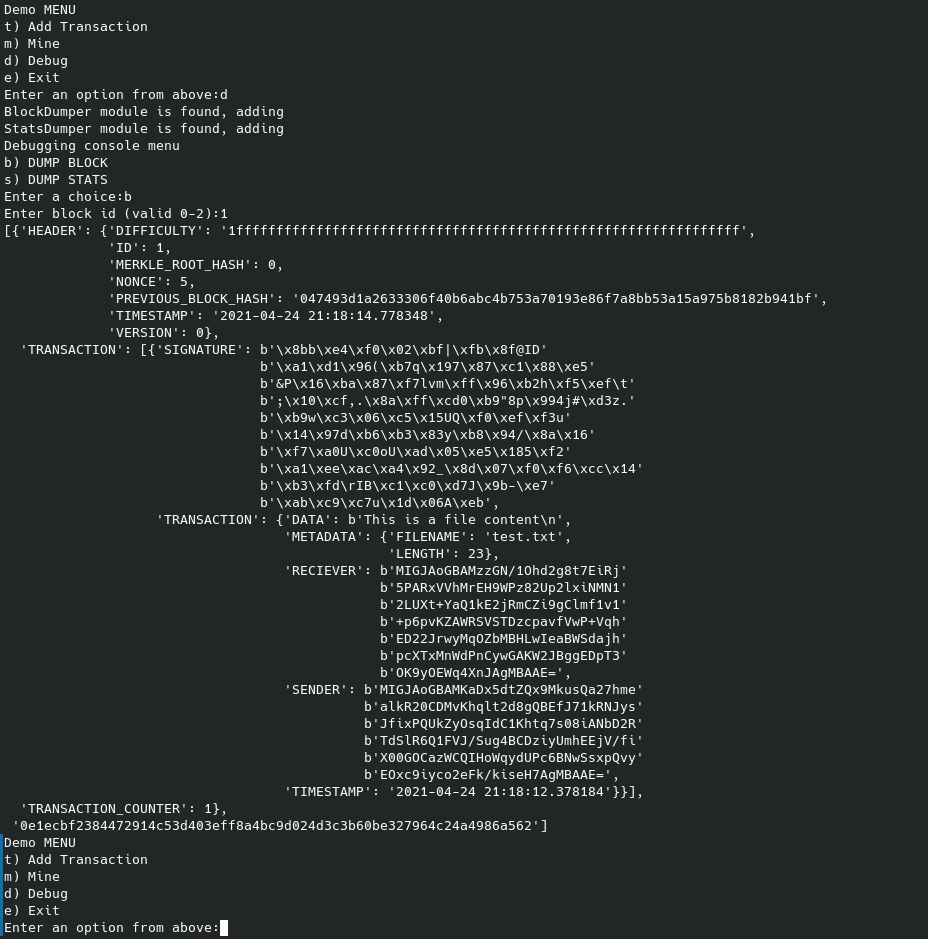
\includegraphics[width=0.7\linewidth]{ViewBlock}
	\caption{Viewing a Block}
	\label{fig:viewblock}
\end{figure}
\begin{figure}[h!]
	\centering
	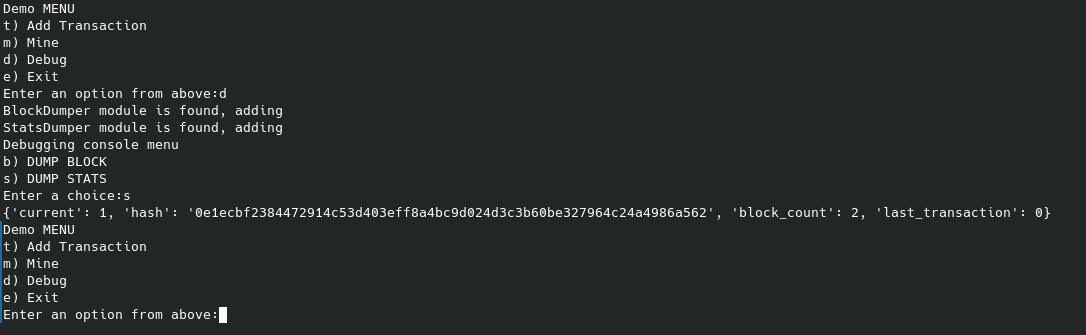
\includegraphics[width=0.7\linewidth]{ViewStats}
	\caption{Viewing stats}
	\label{fig:viewstats}
\end{figure}

\section{Conclusion}
Blockchain based data storage for verification of validity and authenticity of documents is hence proven to be a viable alternative to hologram and other type of conventional verification. It is hard to forge a data which has been added to the block chain and considerable number of blocks have been added on top of the block. This makes it a perfect candidate for replacing the conventional verification system. This system is transparent means that any person can check if a given document is valid. One of the downfalls of this approach is that it is a violation of privacy as anyone with enough information can traverse the whole network and assemble all the documents which are related to a person thereby causing a threat to the person. Therefore, this idea needs to be improved upon for inclusion of privacy. There will always be a tradeoff between privacy and security. It is the duty of the government and the citizens to decide what kind of a system they want, a more robust and secure system which has no privacy or a private system where security can be compromised as it is not easy to verify a person’s identity thereby increasing the chance of identity theft. 

\section*{References}

Please number citations consecutively within brackets \cite{b1}. The 
sentence punctuation follows the bracket \cite{b2}. Refer simply to the reference 
number, as in \cite{b3}---do not use ``Ref. \cite{b3}'' or ``reference \cite{b3}'' except at 
the beginning of a sentence: ``Reference \cite{b3} was the first $\ldots$''

Number footnotes separately in superscripts. Place the actual footnote at 
the bottom of the column in which it was cited. Do not put footnotes in the 
abstract or reference list. Use letters for table footnotes.

Unless there are six authors or more give all authors' names; do not use 
``et al.''. Papers that have not been published, even if they have been 
submitted for publication, should be cited as ``unpublished'' \cite{b4}. Papers 
that have been accepted for publication should be cited as ``in press'' \cite{b5}. 
Capitalize only the first word in a paper title, except for proper nouns and 
element symbols.

For papers published in translation journals, please give the English 
citation first, followed by the original foreign-language citation \cite{b6}.

\begin{thebibliography}{00}
\bibitem{b1} G. Eason, B. Noble, and I. N. Sneddon, ``On certain integrals of Lipschitz-Hankel type involving products of Bessel functions,'' Phil. Trans. Roy. Soc. London, vol. A247, pp. 529--551, April 1955.
\bibitem{b2} J. Clerk Maxwell, A Treatise on Electricity and Magnetism, 3rd ed., vol. 2. Oxford: Clarendon, 1892, pp.68--73.
\bibitem{b3} I. S. Jacobs and C. P. Bean, ``Fine particles, thin films and exchange anisotropy,'' in Magnetism, vol. III, G. T. Rado and H. Suhl, Eds. New York: Academic, 1963, pp. 271--350.
\bibitem{b4} K. Elissa, ``Title of paper if known,'' unpublished.
\bibitem{b5} R. Nicole, ``Title of paper with only first word capitalized,'' J. Name Stand. Abbrev., in press.
\bibitem{b6} Y. Yorozu, M. Hirano, K. Oka, and Y. Tagawa, ``Electron spectroscopy studies on magneto-optical media and plastic substrate interface,'' IEEE Transl. J. Magn. Japan, vol. 2, pp. 740--741, August 1987 [Digests 9th Annual Conf. Magnetics Japan, p. 301, 1982].
\bibitem{b7} M. Young, The Technical Writer's Handbook. Mill Valley, CA: University Science, 1989.
\end{thebibliography}
\section{Appendix}
\href{https://github.com/ABHIRAMSHIBU/BlockChainDataStore}{Github}
\end{document}
